%!TEX root = ../thesis.tex
\chapter{Experiments}
In this chapter, both proposed heterogeneous pc-stable algorithm approaches are evaluated. Furthermore, two different systems are used for the evaluation to elaborate the hardware dependency of the heterogeneous version.

\section{Setup}
The dataset the experiments use for computation is based on the dataset used in the experiments of Perscheid et al. \cite{perscheidIntegrativeGeneSelection2018}. The dataset is taken from The Cancer Genome Atlas (TCGA) \cite{weinsteinCancerGenomeAtlas2013}. Genes with more than 30\% missing values are filtered out. The remaining data is normalized and log-transformed. The original dataset consists of 55 573 variables. While the run-time of the PC stable algorithm grows exponentially with the variable count, subsets of the dataset are used for evaluation. The subset sizes chosen for the evaluation are 1000 variables, 10 000 variables, and 45 000 variables. The 1000 variables dataset is used to represent small datasets and will be called TCGA-1000. The 10 000 variables dataset is a large dataset that does not fill the memory of the system's GPU. The 45 000 variables dataset is therefore used to show the effects of GPU memory overflow on the algorithms execution time in this evaluation.

\begin{figure}[h]
  \caption{System 1 Architektur - Delos}
  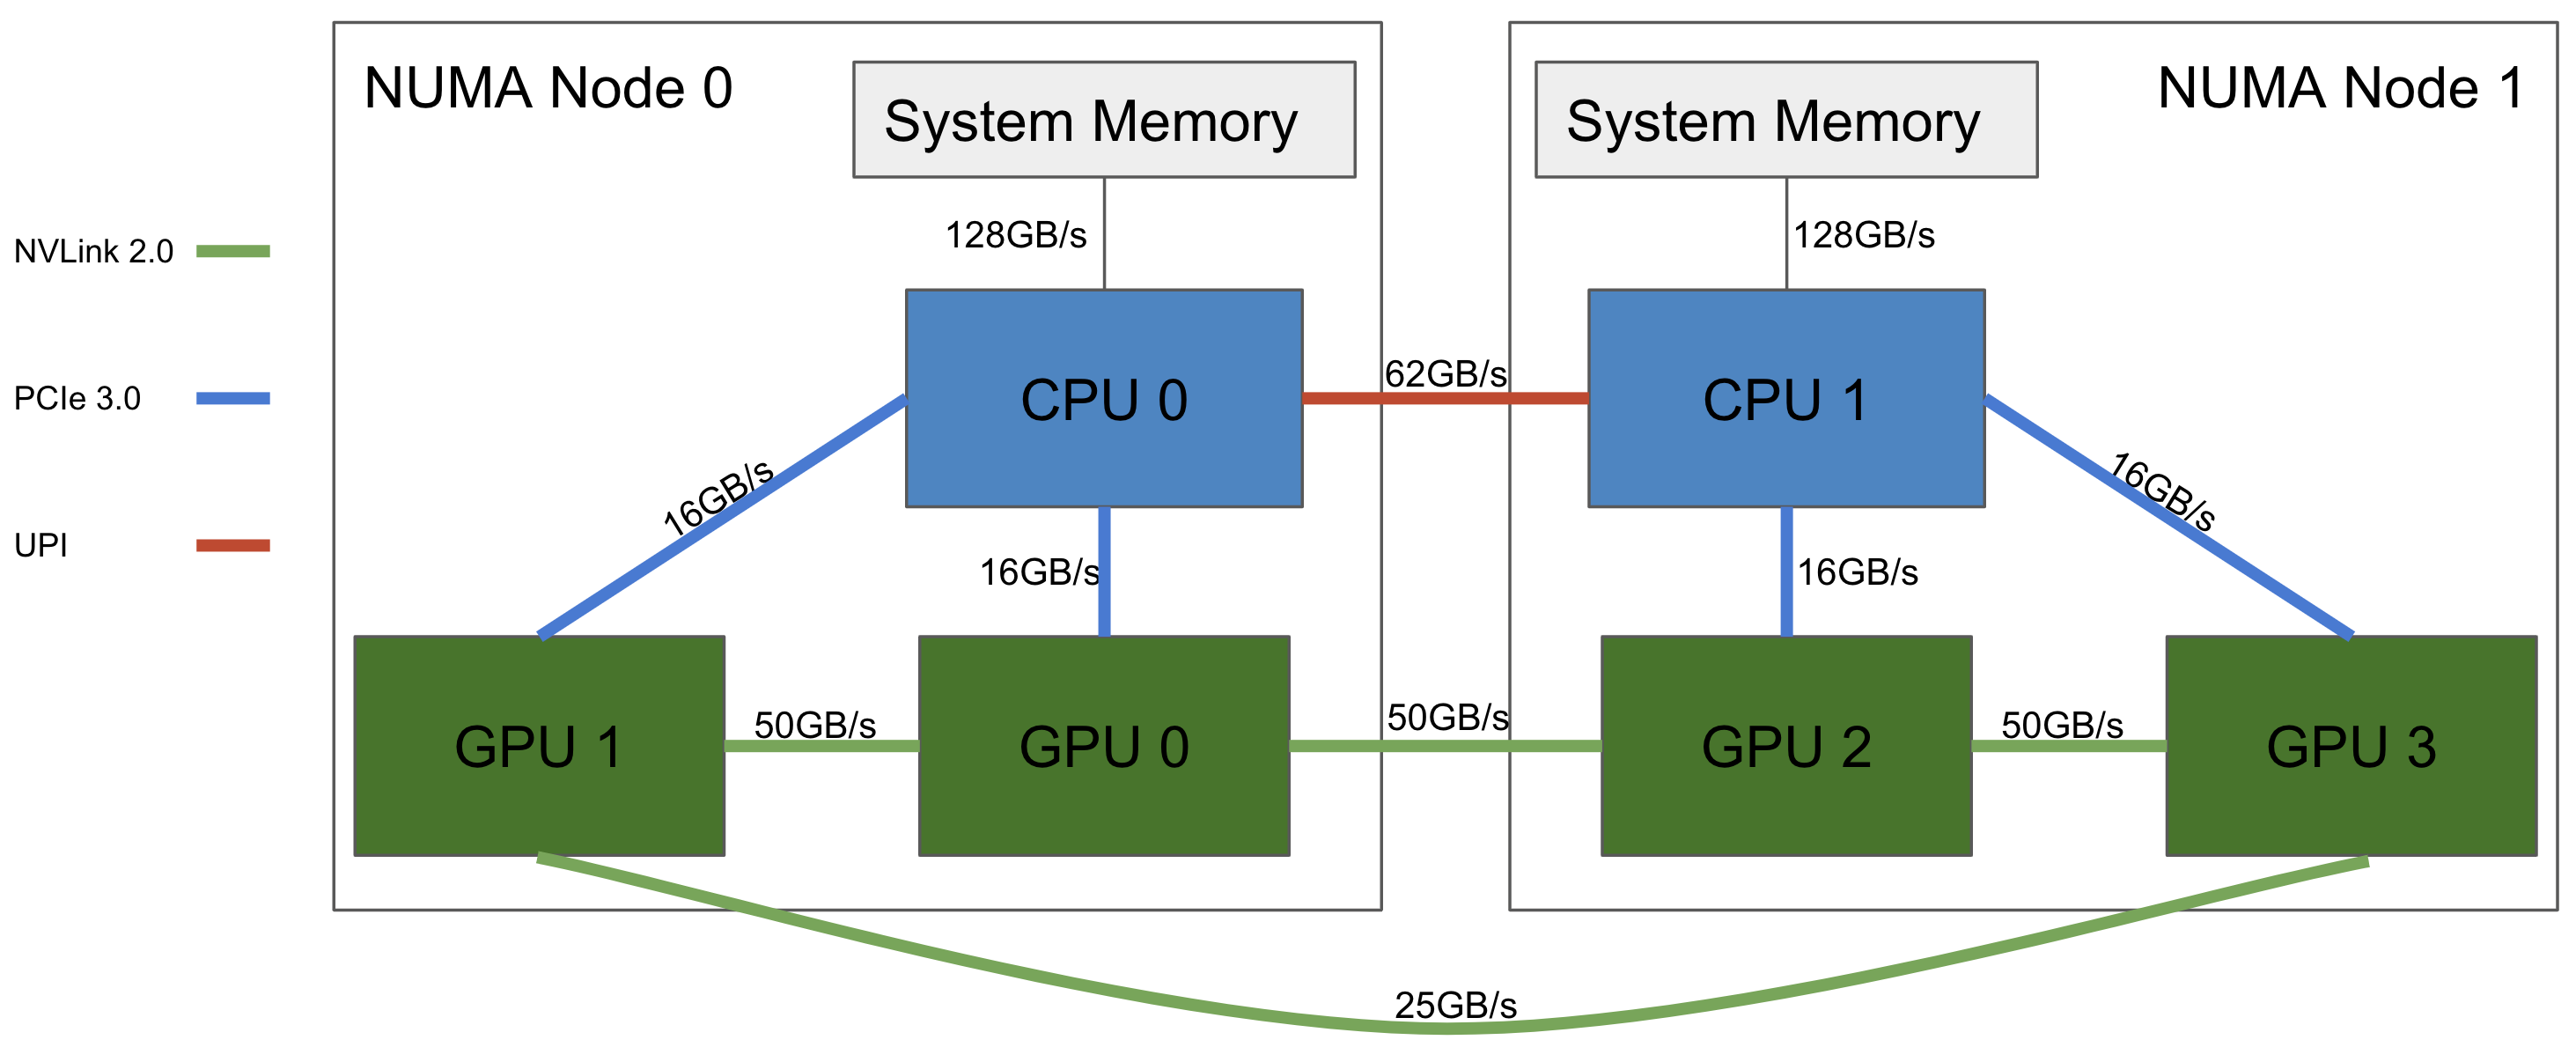
\includegraphics[width=\textwidth]{figures/delos_system_arch.png}
  \centering
  \label{fig:delos_arch}
\end{figure}

Two different systems are used for the evaluation. One system, which will be called Delos \ref{fig:delos_arch} in the following, consists of 4 Nvidia Tesla V100 GPUs with each 32GB of SXM2 memory and 2 Intel Xeon Gold 6148 CPUs with each 755GB of DDR4 memory. The Tesla V100 GPU clock rate is 1,53 GHz. It contains 80 Streaming Multiprocessors which each can execute a maximum of 2048 threads concurrently \cite{NVIDIATESLAV1002017}. The Intel Xeon Gold 6148 has 20 cores with a clock rate maximum of 3,70 GHz. Each core has two so-called hyper threads so that the CPU can execute 40 threads concurrently.

The second system, which will be called AC922 in the following, is a high-performance computing system developed in collaboration with IBM and Nvidia \cite{caldeiraIBMPowerSystem}. It incorporates the same GPUs as the Delos system (4xNvidia Tesla V100) and two IBM Power9 processors. Each Power9 processor has 16 cores with a clock rate maximum of 4 GHz, which, by using SMT4 multithreading, can execute 64 threads concurrently. 256GB DDR4 RAM is connected to each CPU.

Through the collaboration of IBM and Nvidia, the interconnect between a CPU and GPU in this system is NVLINK \cite{NVLink2021, zargesEvaluationOnNodeGPU} with a bandwidth of 150GB/s in contrast to the Delos PCIe 3.0 16GB/s interconnect. NVLINK is also faster latency wise \cite{liEvaluatingModernGPU2020}. The latency and throughput differences of both systems allow evaluating bottlenecks regarding interconnect speed in this heterogeneous computation scenario.
Furthermore the collaboration brings other features which a heterogeneous computing application can benefit from, such as Adress Translation Services \cite{ibmpower9nputeamFunctionalityPerformanceNVLink2018} unifying the GPU and CPU page table, native atomics support for system wide accessible memory and direct GPU memory access by the CPU \cite{UNIFIEDMEMORYP9}.

The following experiments only use one GPU for execution, even if the proposed algorithm can be executed on multiple GPUs at once. Therefore parameters, such as GPU-GPU memory handling and interconnect technology, do not influence the CPU-GPU computation results. Some benchmarks are pinned to the NUMA node closest to the executing GPU to limit interconnect effects not related to the direct CPU-GPU connection. Both systems' CPUs are each directly connected to two GPUs, whichs means using only half the cores and memory while NUMA pinned. The largest dataset being used with the size of 36GB$\sim$ will not be the limiting factor for the CPU's associated memory of 755GB on Delos and 256GB on AC922. On the other hand, 36GB$\sim$ of data will fill the GPU's memory of 32GB which is intentional behavior as said above.

The following table shows the tools and libraries used for the experiments:
\begin{table}[h!]
  \centering
  \begin{tabular}{||c | c||} 
   \hline
   Delos & AC922 \\ [0.5ex] 
   \hline\hline
   GCC 8.4.0 & GCC 8.3.1 \\
   CUDA 11.3 & CUDA 11.3 \\ 
   CMake 3.20.2 & CMake 3.20.2 \\
   Armadillo 10.5.1 & Armadillo 10.5.1 \\
   Boost 1.65.1 & Boost 1.76.0 \\ [1ex]
   \hline
  \end{tabular}
  \caption{Tools and libraries and their versions used in the experiments}
  \label{table:libversions}
\end{table}

Further the following flags were passed to GCC on the systems:
\begin{itemize}
  \item Delos: -O3 -DNDEBUG -march=native -mtune=native
  \item AC922: -O3 -DNDEBUG -flto -fpeel-loops -funroll-loops -ftree-vectorize -ffast-math -mcpu=power9 -mtune=power9
\end{itemize}
The flags used on the AC922 system are recommended by IBM for optimized binaries \cite{LinuxIBMPower}. NVCC, the Nvidia CUDA compiler, gets passed the same flags on both systems (-O3 -DNDEBUG -lineinfo) and additionally CMake autmatically sets the correct flags to compile for best optimization on the V100 architecture.

\section{Benchmarks}
For each system, basic experiments for both approaches are done first to determine the relevance and effectivness of those approaches. To analyze hardware-specific effects on the experiments, more detailed benchmarks are done later, such as tests with a modified thread count used for the CPU execution.
The first approach, which is called pre-balanced, will be tested and compared to the GPU only execution of the algorithm. Additionally, the effect of migrating edges after each level and pinning the execution to some NUMA node is tested as well.

The same tests are then done for the workstealing approach, where a test for atomic usage is added, since atomics are not necessary for this approach and only used so that edges are not processed twice.

Those described experiments are done on both the Delos system and the AC922 system. On the Delos system, further experiments to evaluate the scalability of the approaches are done using larger datasets as said above.

\subsection{Benchmarks Delos}
\begin{table}[H]
  \centering
  \begin{tabular}{||c | c | c | c||} 
   \hline
    & Execution time (ms) & $\Delta$ & $\Delta$ speedup in \% \\ [0.5ex] 
   \hline\hline
   GPU-only & 16290.8 & 0 & - \\
   Pre-Balanced & 15853.8 & -437 & 2,68 \\ 
   No post level migrations & 15821.8 & -469 & 2,96 \\
   NUMA node pinned & 16839.6 & 548,8 & -3,36 \\ [1ex] 
   \hline
  \end{tabular}
  \caption{Pre-Balanced execution time results (Delos)}
  \label{table:preb_delos}
\end{table}
The first experiments using the pre-balanced approach seen in \ref{table:preb_delos} show that there is a slight performance boost of 2,9\% in comparison to the GPU-only variant possible. While pinning the NUMA node, there is even a slow down seen, which tells us two things: First, the missing processing power of the lost cores while pinning the execution is missing, and more cores should help in speeding up the execution. Second, the interconnect bottleneck does not hit the performance in a meaningful way when edges of different rows are processed by GPU and CPU, supported by the little to no effect of migrating edges after level execution. Additionally, the count of rows placed on the CPU by the load balancer had to be tuned carefully for the best performance. The row count balanced on the CPU are in level one and two, 14 rows and in level three and four 8 rows, which is small compared to the maximum of 1000 rows.

This volatility does tuning the pre-balanced approach hard, especially for large datasets where the PC stable algorithm can execute for hours or even days. Multiple tuning executions might not be feasible in such situations, because this threshold might change alot for different datasets which could lead to more sparse rows.



\subsection{Benchmarks AC922}


% - Explain dataset used for testing (TCGA)
%   - Variable size
%   - how sampled
%   - paper (perscheid etc)
% - Show delos as a testing machine
%   - Intel Xeon 
%   - Nvidia  V100
%   - specs
%   - numa nodes
% - Show AC922
%   - Explain why power9 + V100 special
%   - ATS: Malloc is enough
%   - Faster interconnect NVLINK
%     - Comparison between interconnects
%   - Other pros : atomics etc
%   - Explain why this should affect my performance
%   - Compare Power9 to Intel Xeon
% - Show iteration measurements per level
%   - show how many tests and iterations have to be done

% - Measurements of GPU only Code

% - Measurements of Pre-balanced
%   - With, without migrating edges
%   - Different thresholds
%   - Different Dataset sizes
%   - Different omp scheduling methods
%   - Pinning on NUMA nodes
%   - Delos vs AC922
% - Measurements of Workstealing
%   - With, without migrating edges
%   - Different Dataset sizes
%   - Pinning on NUMA nodes
%   - Delos vs AC922

% - Measurements with different Datasets
%   - Iterations
%   - Workstealing Numa 0
%   - Prebalanced
%   - GPU only
